\documentclass[11pt, a4paper]{article}
\input{preamble.tex}
\switchlang{ru}
\begin{document}

\title{1989 "--- Prohance PowerMouse 100}
\date{}
\maketitle
\selectlanguage{russian}
Мышь Prohance PowerMouse 100 была выпущена компанией Prohance Technologies inc. в 1989 году в рамках целого семейства из нескольких мышей и одного трекбола, ориентированных на пользователей электронных таблиц Lotus 1-2-3 (и некоторых других подобных приложений). Концепция Prohance заключается в размещении множества дополнительных кнопок на корпусе, которые, по замыслу разработчиков, избавляют пользователя от необходимости часто перемещать руку с мыши на клавиатуру и обратно. Prohance mouse содержит в передней части корпуса дополнительную функциональную клавиатуру: в данной модели, PowerMouse 100, число кнопок является максимальным и составляет 40 (рис. \ref{fig:ProhancePhoto}). Разместить такое количество кнопок оказалось возможным за счет сильно вытянутого в длину корпуса мыши, похожего на пульт дистанционного управления \cite{livingston}.

\begin{figure}[h]
    \centering
    
\includegraphics[scale=0.47]{1989_prohance_powermouse_100/pic_60.jpg}
    \caption{Изображение Prohance mouse 100}
    \label{fig:ProhancePhoto}
\end{figure}

Как можно увидеть на рис. \ref{fig:ProhanceTopAndBottom}, корпус разделн на три части. Дальняя от пользователя область содержит 28 прямоугольных клавиш, играющих роль цифровой клавиатуры, либо функциональных клавиш, при зажатой клавише <<Fn>>. Средняя часть содержит две узкие длинные кнопки, соответствующие левой и правой кнопкам мыши, а также еще десять маленьких круглых кнопок, назначение которых подписано на сменной пластиковой вставке и может меняться так же, как эта вставка. Наконец, ближняя к пользователю часть корпуса содержит только логотип фирмы-производителя и служит опорой для запястья. На нижней стороне корпуса присутствуют низкофрикционные накладки, табличка с техническими данными и поворотное кольцо-защелка, необходимое, чтобы извлечь шар для чистки. Данный вариант мыши является ранним и датируется 1989 годом \cite{pcmag}.

\begin{figure}[h]
    \centering
    
\includegraphics[scale=0.5]{1989_prohance_powermouse_100/top_60.jpg}
    
\includegraphics[scale=0.5]{1989_prohance_powermouse_100/bottom_60.jpg}
    \caption{Изображение ранней версии Prohance PowerMouse 100, вид сверху и снизу}
    \label{fig:ProhanceTopAndBottom}
\end{figure}

Рисунок \ref{fig:ProhanceTopAndBottom2} демонстрирует более позднюю модификацию мыши, доступную к приобретению в 1992 году \cite{box}. Как можно заметить, в ней не предусмотрено автоматическое дублирование функциональных клавиш клавиатуры, изменено назначение некоторых других кнопок, а также на рисунке можно увидеть несколько вставок: более универсальный вариант по умолчанию, а также версии для работы с электронными таблицами и с текстовыми процессорами.

\begin{figure}[h]
    \centering
    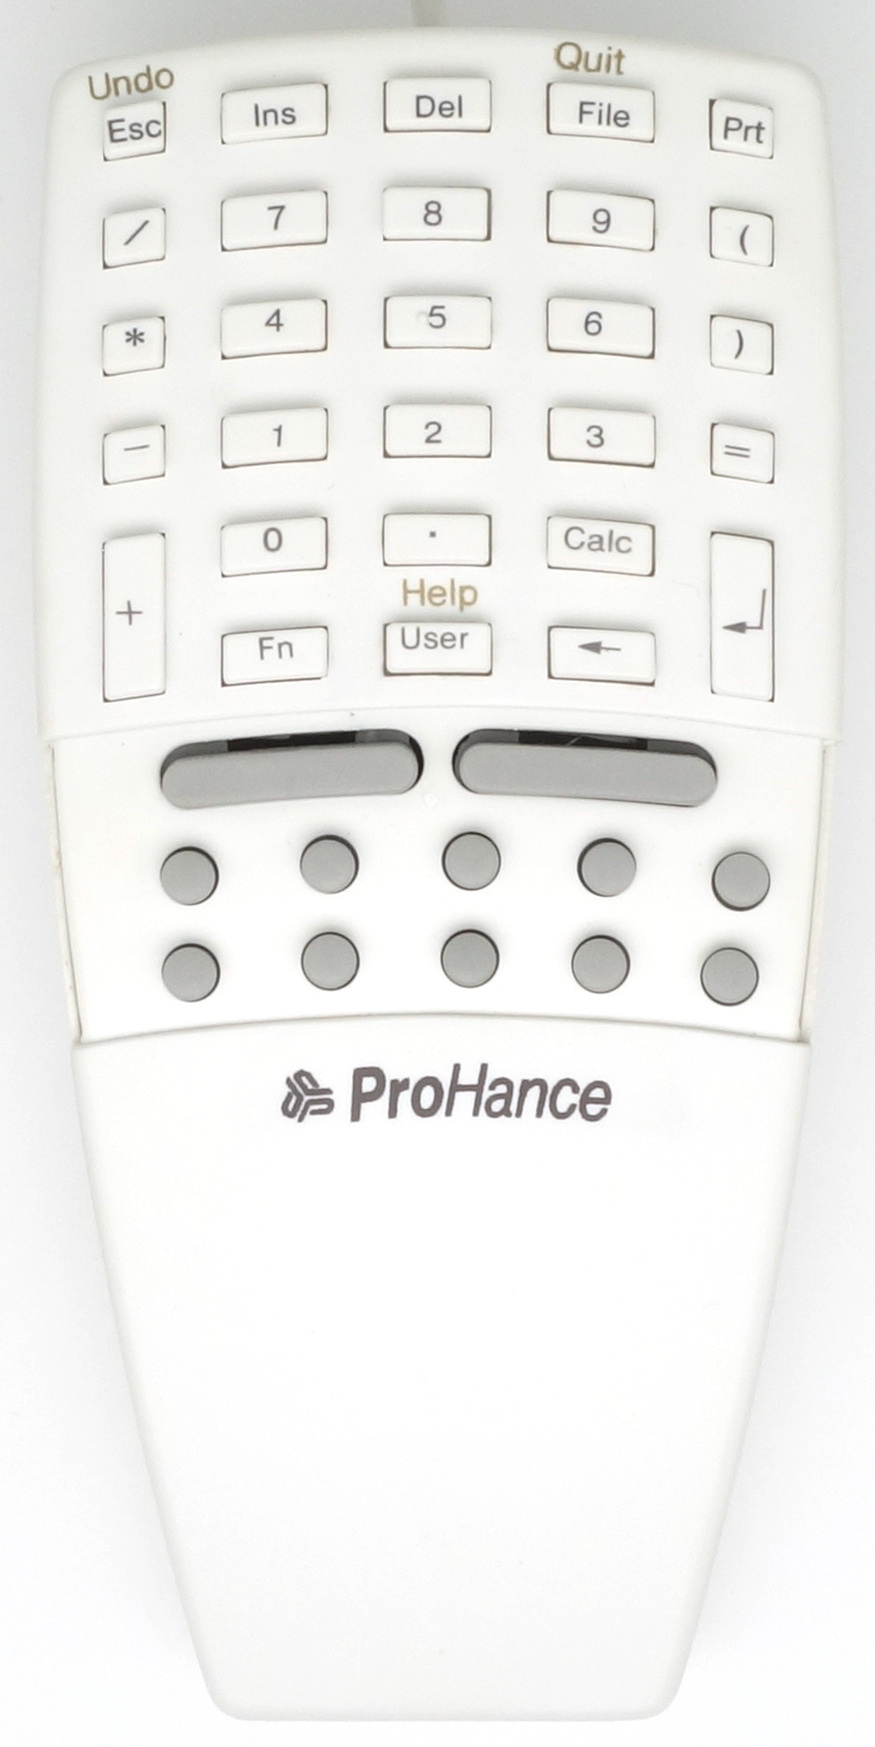
\includegraphics[scale=0.5]{1989_prohance_powermouse_100/top1_30.jpg}
    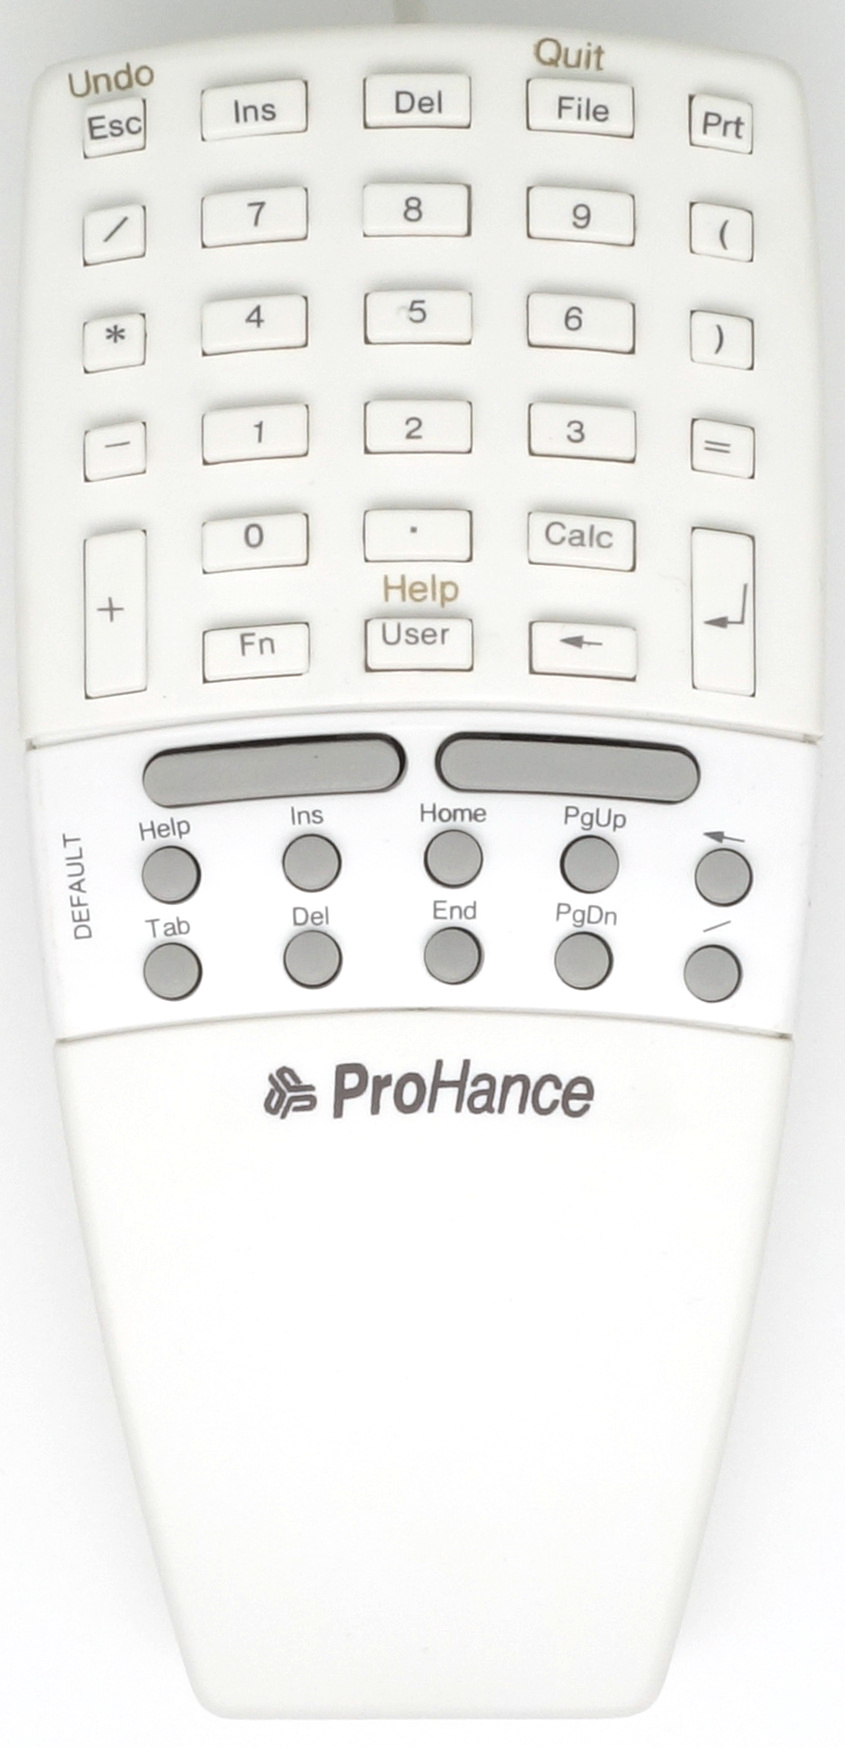
\includegraphics[scale=0.5]{1989_prohance_powermouse_100/top2_30.jpg}
    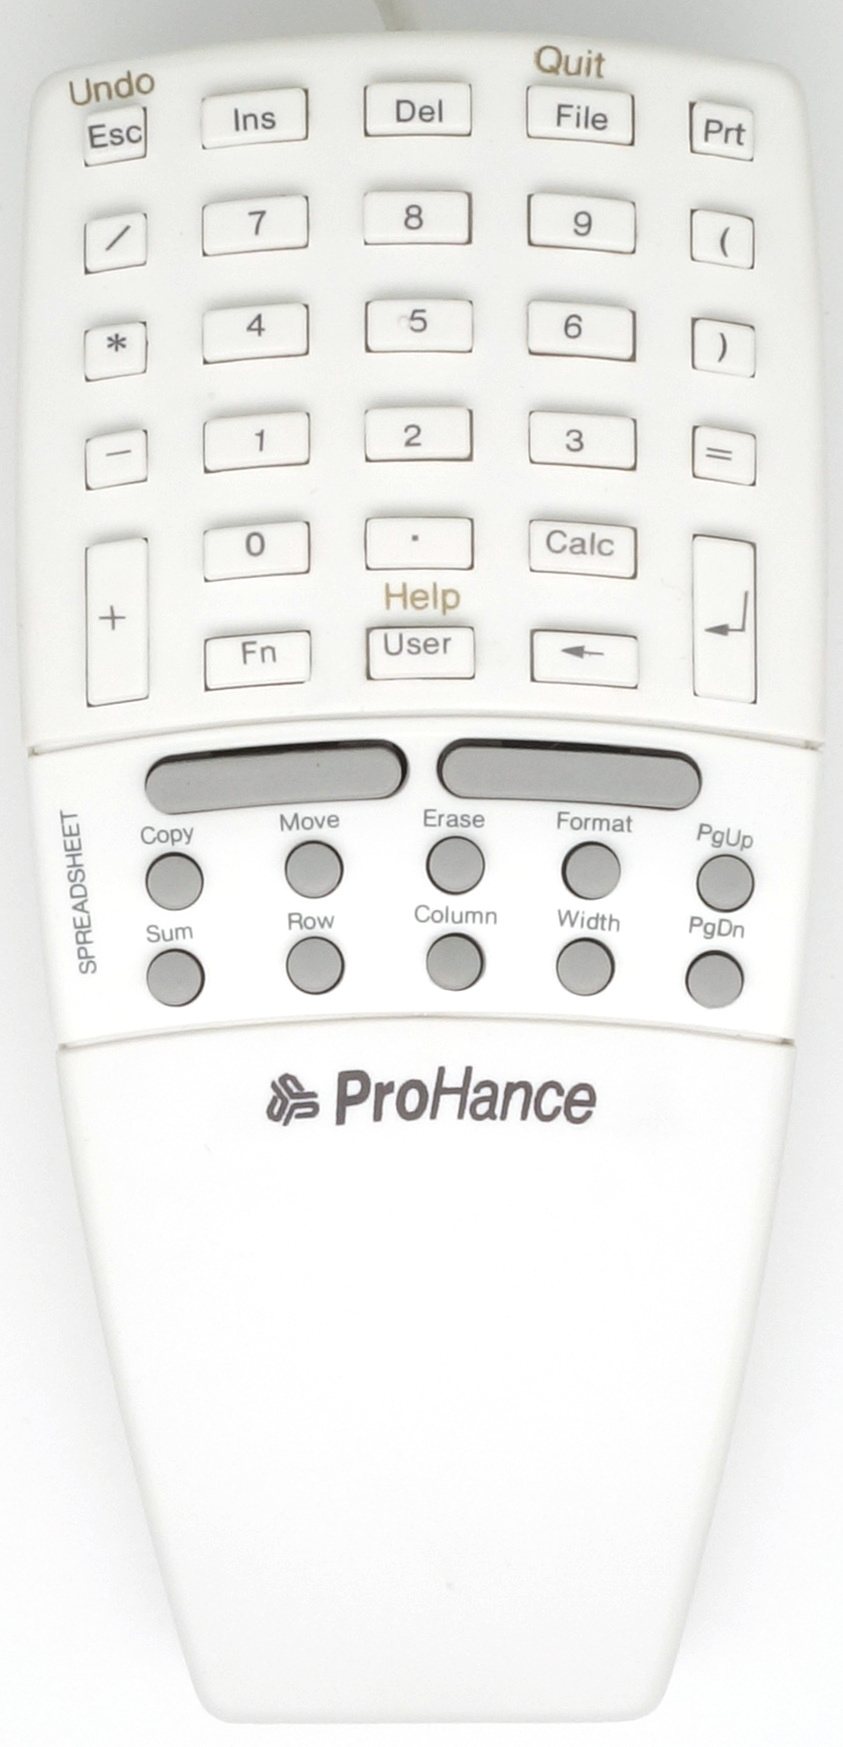
\includegraphics[scale=0.5]{1989_prohance_powermouse_100/top3_30.jpg}
    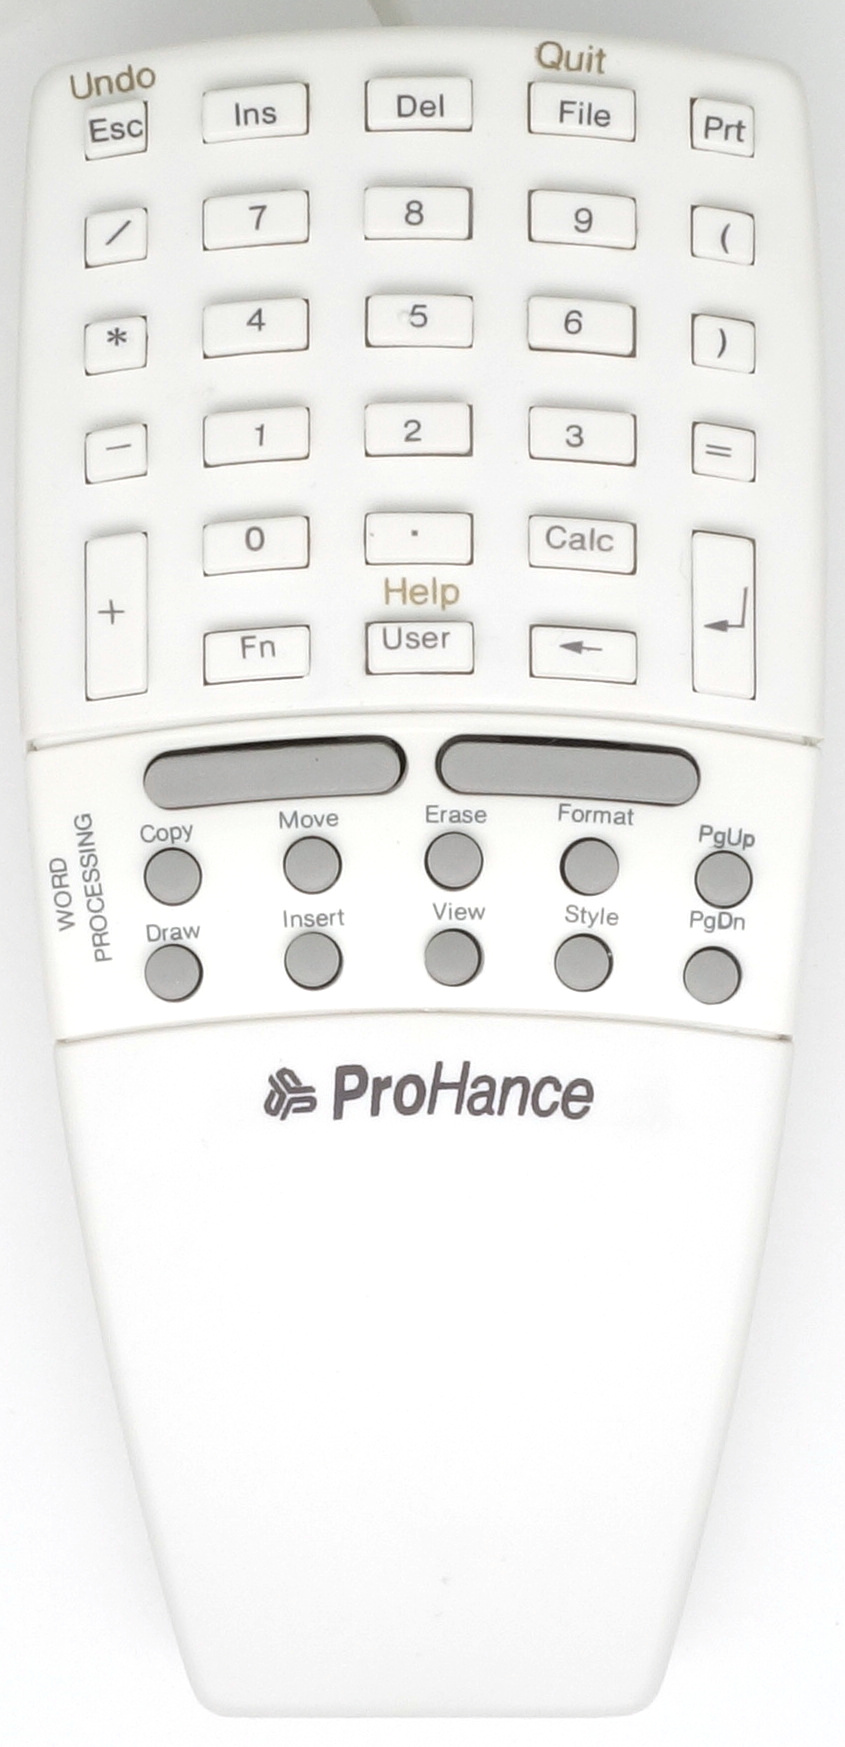
\includegraphics[scale=0.5]{1989_prohance_powermouse_100/top4_30.jpg}
    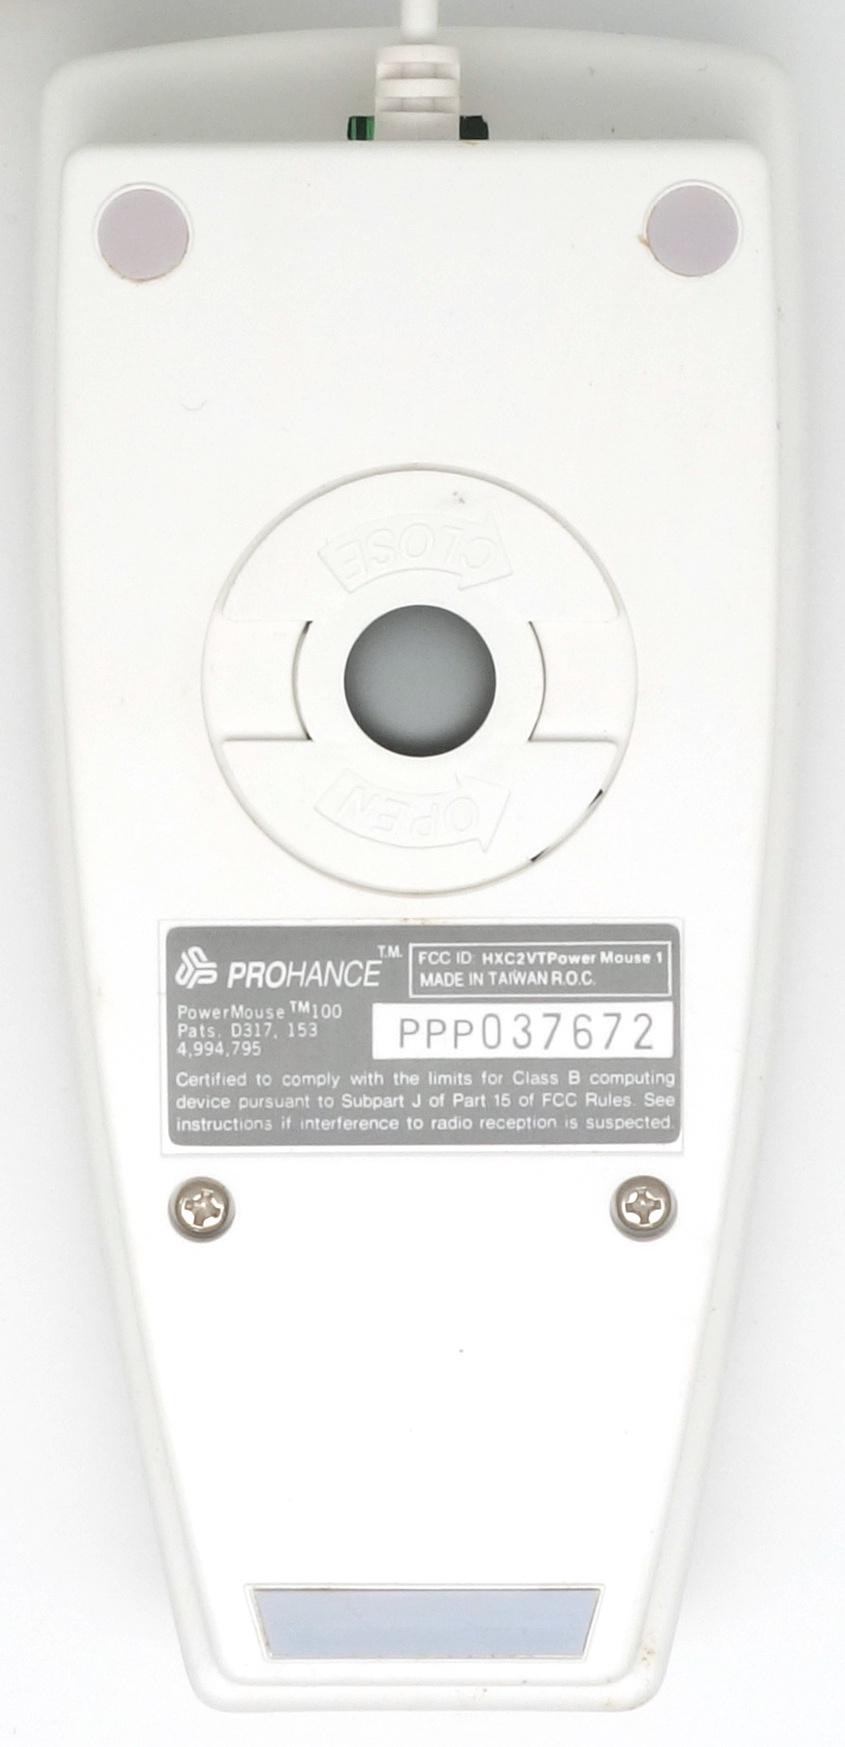
\includegraphics[scale=0.5]{1989_prohance_powermouse_100/bottom1_30.jpg}
    \caption{Изображение поздней версии Prohance PowerMouse 100, вид сверху и снизу}
    \label{fig:ProhanceTopAndBottom2}
\end{figure}

В качестве поддерживаемых приложений в версии 1992 года Prohance упоминает <<текстовые редакторы, электронные таблицы, САПР, настольные издательские системы, базы данных, графические редакторы и многое другое>>. Их поддержка заключается в том, что при нажатии функциональной клавиши мыши драйвером генерируется заданная последовательность событий клавиатуры и мыши, то есть фактически нажатие приводит к выполнению макрокоманды. Конфигурационное программное обеспечение Prohance, работающее под управлением MS DOS, позволяет переключать наборы этих макрокоманд, а также создавать новые \cite{manual}: 6 определяемых задач для каждой кнопки (с использованием клавиш Shift, Ctrl, Alt и т. д.). В остальном устройство действует как обычная мышь. В \cite{prohance} отмечается, что в ранней версии драйвера содержались ошибки, приводившие к неадекватной работе мыши в Microsoft Word (даже ее незначительное перемещение приводило к пролистыванию страниц), исправленные в обновленной версии. Также отмечалась некоторая программная несовместимость с драйвером мыши Microsoft, приводившая к неработоспособности мыши в части приложений. Драйвер также позволял задавать через конфигурационный файл уровень чувствительности мыши, однако функция динамического регулирования ускорения мыши предусмотрена не была.

\begin{figure}[h]
    \centering
    
\includegraphics[scale=0.34]{1989_prohance_powermouse_100/size_30.jpg}
    \caption{Изображение Prohance Mouse 100 на размерном коврике с шагом сетки 1~см}
    \label{fig:ProhanceSize}
\end{figure}

Размеры корпуса Prohance PoverMouse 100 (рис. \ref{fig:ProhanceSize}) сказываются на ее эргономике не лучшим образом, однако это не единственная проблема мыши. Не менее важным недостатком является размер кнопок: как основные кнопки мыши, так и дополнительные клавиши Prohance имеют очень маленькую площадь. Колпачки клавиш резиновые, как у микрокалькулятора, и издают едва слышный клик при нажатии (при этом их запас хода уменьшает вероятность случайного срабатывания).

Сами по себе колпачки кнопок не содержат тактильных или визуальных отличительных признаков. Это особенно проблемно для функциональных клавиш: они имеют круглые колпачки одинакового размера, поэтому перед нажатием нужно внимательно следить за правильным положением пальцев. Накладки, размещаемые поверх функциональной клавиатуры, позволяют выполнять визуальную идентификацию клавиш в различных режимах работы. Однако надписи на них достаточно мелкие, перекрываются пальцами, и нетренированному пользователю приходится пристально их рассматривать, чтобы найти нужную (разница в размерах подушечки пальца и функциональной кнопки хорошо видна на рис. \ref{fig:ProhanceHand}).

\begin{figure}[h]
    \centering
    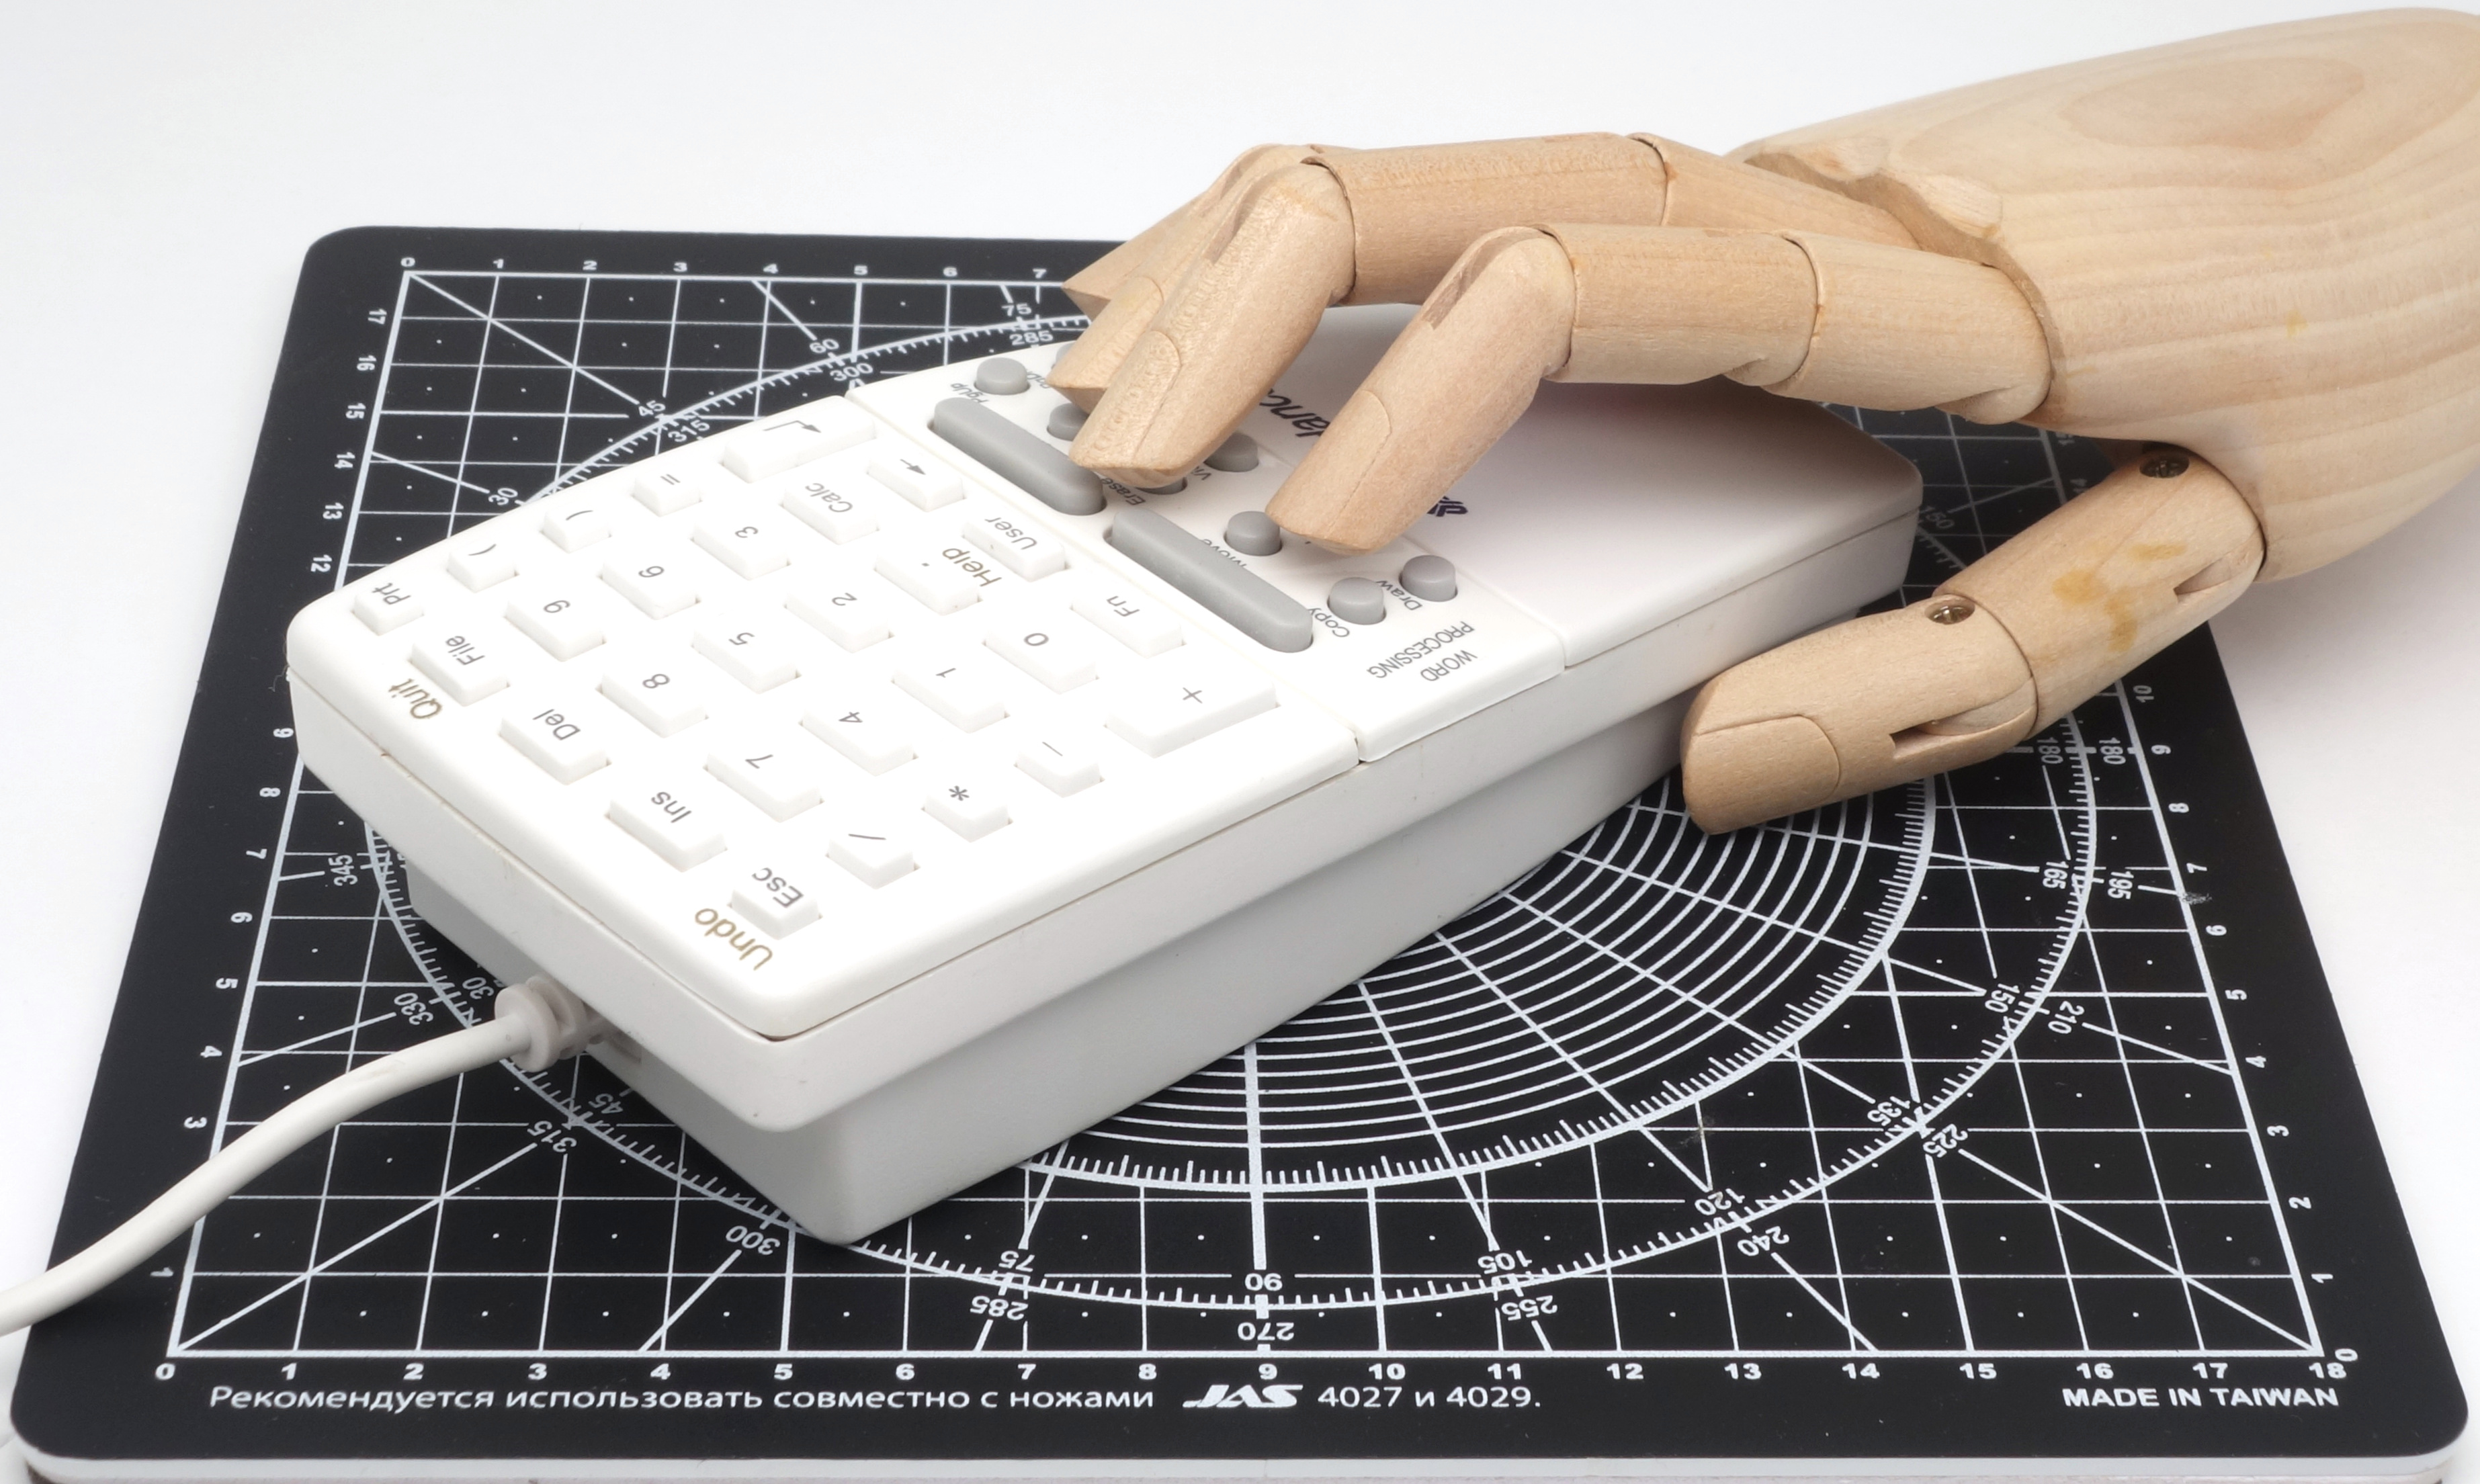
\includegraphics[scale=0.4]{1989_prohance_powermouse_100/hand2_15.jpg}
    \caption{Изображение Prohance Mouse 100 с моделью руки человека}
    \label{fig:ProhanceHand}
\end{figure}

Компания-производитель позиционировала как эргономическое преимущество то, что пользователям было <<больше не нужно тратить время или терять концентрацию, постоянно переключаясь между клавиатурой и выпадающими меню>> \cite{box}. Однако взамен им приходилось мириться с необходимостью нажимать на чрезвычайно узкие левую и правую кнопки мыши и вглядываться в мелкие надписи между клавишами, что не прибавляло мыши положительных отзывов.

\begin{figure}[h]
    \centering
    
\includegraphics[scale=0.8]{1989_prohance_powermouse/inside_60.jpg}
    \caption{Изображение Prohance в разобранном виде}
    \label{fig:ProhanceInside}
\end{figure}

Мышь в разобранном виде показана на рис. \ref{fig:ProhanceInside}. Как можно видеть, она представляет собой типичную для начала 90-х годов оптомеханическую конструкцию, а блок кнопок и функциональных клавиш выполнен на отдельной печатной плате и является миниатюрной мембранной клавиатурой, аналогичной устанавливаемым в карманных микрокалькуляторах.

\begin{thebibliography}{9}
\bibitem{livingston} Livingston B. Genetically engineered mice run amok at Windows World // InfoWorld, Vol. 15, Iss. 21, May 24, 1989. - p. 34. \url{https://books.google.by/books?id=PTsEAAAAMBAJ&lpg=PA34&dq=prohance%20mouse&hl=ru&pg=PA34#v=onepage&q=prohance%20mouse&f=false}
\bibitem{pcmag} Mouse Integrates Numeric Keypad, Programmable Keys // PC Magazine, V. 8, Iss. 12, June 27, 1989. - P. 56. \url{https://archive.org/details/PC-Mag-1989-06-27/page/n57/mode/2up}
\bibitem{prohance} Gruman G. What price mice? // Infoworld, V. 12, No. 17, April 23, 1990. - P. 63-69. \url{https://books.google.by/books?id=LTsEAAAAMBAJ&lpg=PA63&ots=GzwI8rKvl3&dq=%22prohance%20powermouse%22&pg=PA63#v=onepage&q&f=false}
\bibitem{box} Prohance PowerMouse 100 [the box] \url{raw.githubusercontent.com/fiowro/mouses/main/source/OCR/prohance_powermouse_100_box.pdf}
\bibitem{manual} Prohance PowerMouse and PowerTrack User's guide \url{raw.githubusercontent.com/fiowro/mouses/main/source/OCR/prohance_powermouse_powertrack_manual.pdf}
\end{thebibliography}
\end{document}
